\documentclass[11pt,letterpaper]{article}
\usepackage[lmargin=1in,rmargin=1in,tmargin=1in,bmargin=1in]{geometry}
\usepackage{../style/homework}
\usepackage{../style/commands}
\setbool{quotetype}{false} % True: Side; False: Under
\setbool{hideans}{true} % Student: True; Instructor: False

% -------------------
% Content
% -------------------
\begin{document}

\homework{17: Due 12/01}{There is no branch of mathematics, however abstract, which may not some day be applied to phenomena of the real world.}{Nikolai Lobachevsky}

% Problem 1
\problem{10} Showing all your work and as accurately as possible, plot the region given by the inequalities below:
	\[
	\begin{aligned}
	x_1 + &x_2 \leq 5 \\
	x_1 &\leq 3 \\
	x_1, & \, x_2 \geq 0 \\
	\end{aligned}
	\]
Is the region bounded or unbounded?
	\[
	\fbox{
	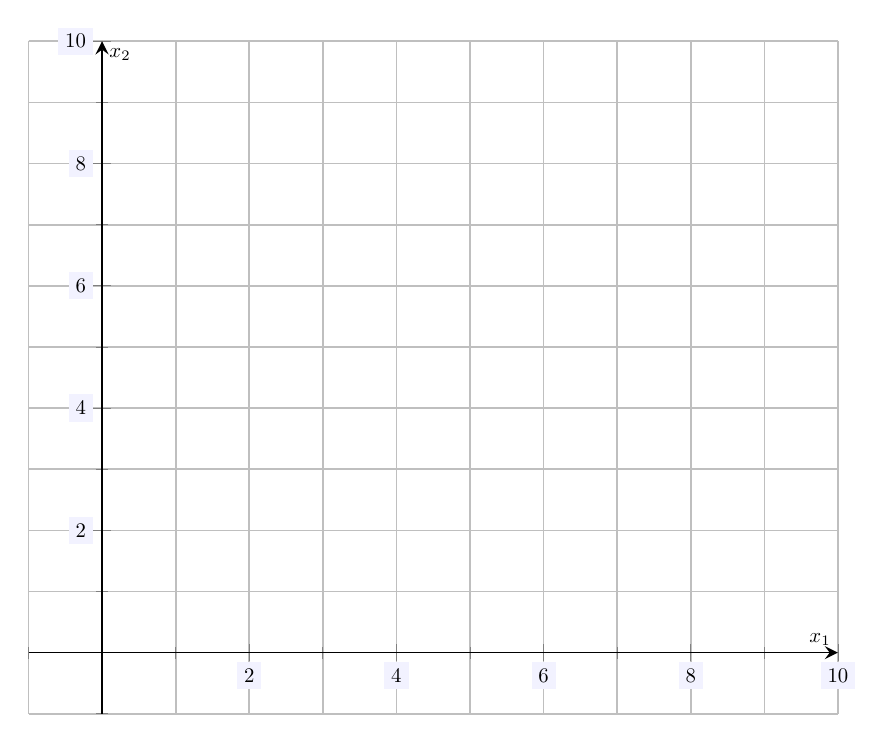
\begin{tikzpicture}[scale=1.5,every node/.style={scale=0.5}]
	\begin{axis}[
	grid=both,
	axis lines=middle,
	ticklabel style={fill=blue!5!white},
	xmin= -1, xmax=10,
	ymin= -1, ymax=10,
	xtick={0,2,4,6,8,10},
	ytick={0,2,4,6,8,10},
	minor tick = {-1,0,1,...,10},
	xlabel=\(x_1\),ylabel=\(x_2\),
	]
	\end{axis}
	\end{tikzpicture}
	}
	\]



\newpage



% Problem 2
\problem{10} Showing all your work and as accurately as possible, plot the region given by the inequalities below:
	\[
	\begin{aligned}
	x_1 + 2x_2 &\geq 7 \\
	x_1 + x_2 &\geq 5 \\
	x_1, x_2 &\geq 0
	\end{aligned}
	\]
Is the region bounded or unbounded?
	\[
	\fbox{
	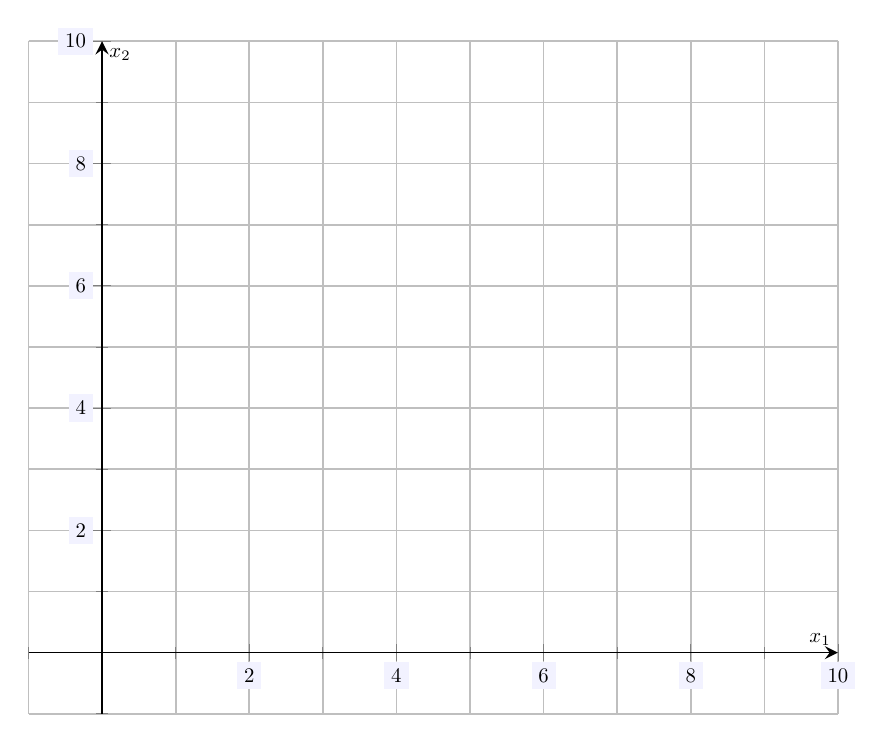
\begin{tikzpicture}[scale=1.5,every node/.style={scale=0.5}]
	\begin{axis}[
	grid=both,
	axis lines=middle,
	ticklabel style={fill=blue!5!white},
	xmin= -1, xmax=10,
	ymin= -1, ymax=10,
	xtick={0,2,4,6,8,10},
	ytick={0,2,4,6,8,10},
	minor tick = {-1,0,1,...,10},
	xlabel=\(x_1\),ylabel=\(x_2\),
	]
	\end{axis}
	\end{tikzpicture}
	}
	\]


\end{document}